\section{Sallen-Key aktive filtre}

Til anti aliasing filtrene anvendes aktive filtre, dette er valgt da det så ikke er
nødvendigt at skulle anvende spoler, da disse ofte fylder meget og heller ikke er
tilgængelige i et lige så bredt omfang, som kondensatorer og modstander, på SDU.
Samtidigt er det nemt at implementere da systemet i forvejen har strømforsyning til
mikroprocessoren, som kan anvendes til filtrenes operationsforstærker.

Her er det valgt at anvende Sallen-Key lav pas biquads,
da disse kan realiseres ved hjælp af flere forskellige designmetoder, præsenteret 
i læreborgen 'Analog filters, second edition'\cite{KendallSu}.
En generisk Sallen-Key lavpas biquad ser ud som i figur(\ref{fig:sklpbq}).

\begin{figure}[H]
	\centering
	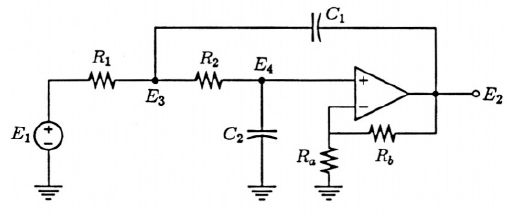
\includegraphics[width=\textwidth]{billeder/sklpbq}
	\caption{Sallen-Key lowpass biquad \cite{KendallSu}}
	\label{fig:sklpbq}
\end{figure}

Det blev valgt at anvende design metode 4 fra litteraturen, minimum sensitivitet.
Denne designmetode gør filteret mindre sensitiv over for variationer i komponenter ved bl.a.
at anvende enheds forstærkning for derfor at undvære $R_a$ og $R_b$.
Det vælges at $R_1 = R_2$, herefter findes $C_1$ og $C_2$ ved hjælp af ligning \ref{eq:dm4c1} og \ref{eq:dm4c2}.

\vspace{15pt}

\begin{minipage}{0.5\linewidth}
	\begin{equation}
	\label{eq:dm4c1}
		C_1 = \frac{2Q}{\omega_0}
	\end{equation}
\end{minipage}
\begin{minipage}{0.5\linewidth}
	\begin{equation}
	\label{eq:dm4c2}
	C_2 = \frac{1}{2Q\omega_0}
	\end{equation}
\end{minipage}

\vspace{15pt}

Det kan så ses at denne designmetode dog kommer på bekostningen af en stor spredning i
kondensator værdierne, som stiger afhængigt af filterets Q-værdi, som ses i ligning
\ref{eq:kondspred}.

\begin{equation}
\label{eq:kondspred}
	\frac{C_1}{C_2} = 4Q^2
\end{equation}



